\section{SCARS Documentation}\label{sec:documentation}
    The purpose of this chapter is to provide the user with information about SCARS Toolbox documentation. While most of the structure and architecture of SCARS is described in \autoref{toolbox:architecture}, the purposes and operation principles of major blocks are shown in \autoref{sec:space_mechanics}, \ref{sec:environment}, \ref{sec:actuators},  \ref{sec:sensors},   and the instructions on how to use it are provided in \autoref{sec:examples}, some additional explanation might be necessary. 
    
    In following sections contain the descriptions of folder structure in SCARS, the scripts which are shipped along Simulink models and how SCARS uses Simulink model masks to provide easily accessible documentation to the user.
    


    \subsection{Folder Structure}
        \dots\textit{work in progress}\dots
    


    \subsection{MATLAB Scripts}\label{sec:scripts}
        Along with Simulink models, SCARS is shipped with few MATLAB scripts. Their aim is to automate menial tasks that have to be performed by the user. Since the scripts guide the user with interactive prompts, there is no need for detailed documentation, just explanation of their purpose, presented in the list below:
        
        \begin{itemize}
            \item \verb|scarsSetup| - Once run it provides the SCARS Modular Simulation with all necessary variables. Can be copied and edited to initialize the model with parameters chosen by the user.
            \item \verb|getSunPosition| - Provides \textbf{Sun's Position [km]} block with arrays for lookup tables. Has to be run before using said block.
            \item \verb|createSTKFiles| - Exports data from SCARS simulation into STK ephemeris and attitude files.
            \item \verb|getSISOSystem| - Changes the system linearized with Simulink Model Linearizer into \ac{siso} system. Walks the user through the process with series of prompts, hence initially it doesn't require any parameters.
        \end{itemize}
        
        % \dots\textit{work in progress}\dots



    \subsection{Simulink Models Masks}
        Each model included in \ac{scars} Parts Library is masked with Simulink mask\cite{masks}. This allows the user to open custom interface for selected SCARS block, with editable fields for each parameter used in the setup process of that part. Most importantly, masks contain the description of the block. In case of SCARS, if the block represents a piece of hardware, the description contains short explanation of principle of operation of said part, its purpose within AOCS subsystem, notes about parameters, and description of block's inputs and outputs. In this way, majority of SCARS documentation is attached to the model itself, where it is easily accessible. An example of SCARS block mask can be found in figure \autoref{fig:model_mask}.
        
        \begin{figure}[H]
            \centering
            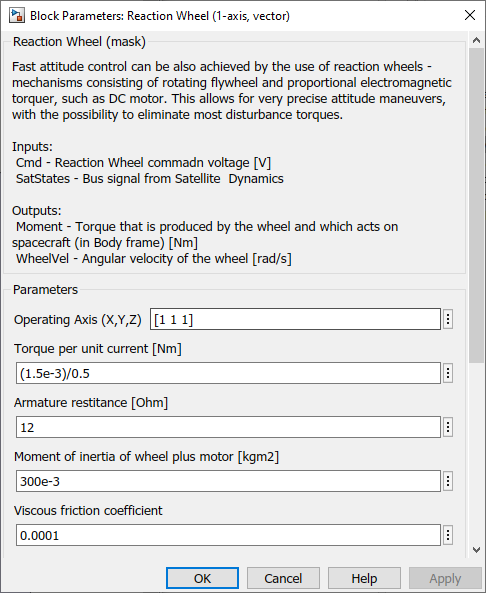
\includegraphics[scale=0.44]{3-documentation/rw_mask.png}
            \caption{SCARS Reaction Wheel block mask}
            \label{fig:model_mask}
        \end{figure}
        
        Also, Simulink masks contain pieces of MATLAB code, which is executed after adding or changing the block. This code allows further customization of the initialization process. For example, \textbf{Reaction Wheel (1 axis, vector)} model transforms the vector given as axis of operation into its norm, "sanitating" user's input. 
        % \dots\textit{description}\dots
